%%%%%%%%%%%%%%%%%%%%%%%%%%%%%%%%%%%%%%%%%
% University/School Laboratory Report
% LaTeX Template
% Version 3.1 (25/3/14)
%
% This template has been downloaded from:
% http://www.LaTeXTemplates.com
%
% Original author:
% Linux and Unix Users Group at Virginia Tech Wiki 
% (https://vtluug.org/wiki/Example_LaTeX_chem_lab_report)
%
% License:
% CC BY-NC-SA 3.0 (http://creativecommons.org/licenses/by-nc-sa/3.0/)
%
%%%%%%%%%%%%%%%%%%%%%%%%%%%%%%%%%%%%%%%%%

%----------------------------------------------------------------------------------------
%	PACKAGES AND DOCUMENT CONFIGURATIONS
%----------------------------------------------------------------------------------------

\documentclass{article}

\usepackage[version=3]{mhchem} % Package for chemical equation typesetting
\usepackage{siunitx} % Provides the \SI{}{} and \si{} command for typesetting SI units
\usepackage{graphicx} % Required for the inclusion of images
\usepackage{natbib} % Required to change bibliography style to APA
\usepackage{amsmath} % Required for some math elements 
\usepackage{hyperref}
\usepackage[a4paper,margin=0.5in]{geometry}
\setlength\parindent{0pt} % Removes all indentation from paragraphs

\renewcommand{\labelenumi}{\alph{enumi}.} % Make numbering in the enumerate environment by letter rather than number (e.g. section 6)

%\usepackage{times} % Uncomment to use the Times New Roman font

%----------------------------------------------------------------------------------------
%	DOCUMENT INFORMATION
%----------------------------------------------------------------------------------------

\title{One Shot Detectors} % Title

\author{Philipp \textsc{Duernay}} % Author name

\date{\today} % Date for the report

\begin{document}
\maketitle
% If you wish to include an abstract, uncomment the lines below
% \begin{abstract}
% Abstract text
% \end{abstract}

%----------------------------------------------------------------------------------------
%	SECTION 1
%----------------------------------------------------------------------------------------
\begin{figure}[h]
	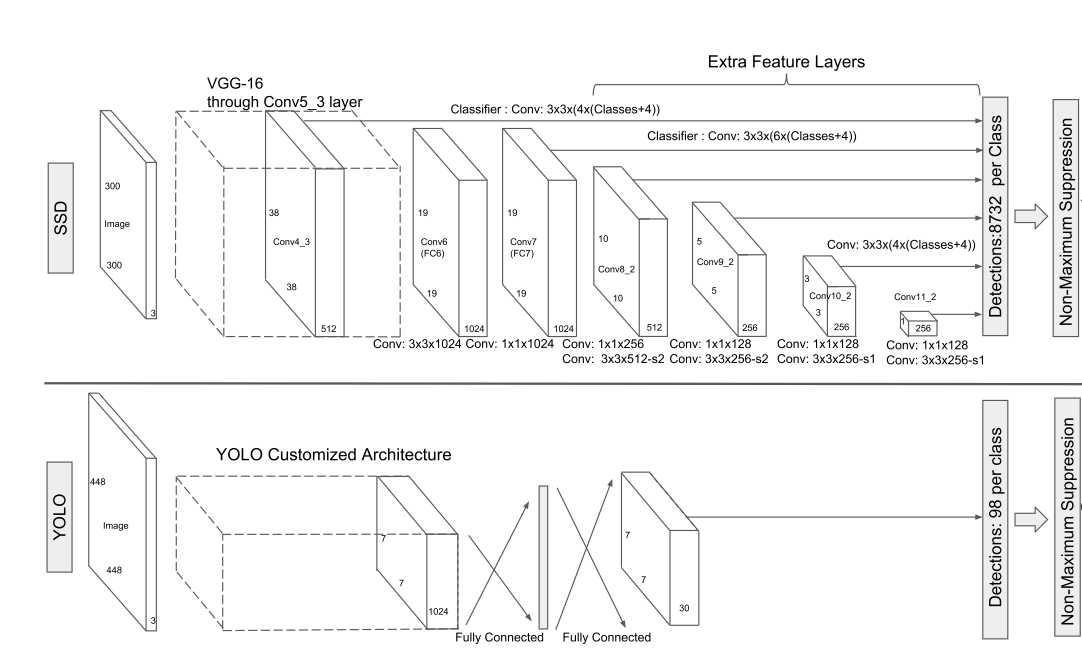
\includegraphics[width=0.9\textwidth]{fig/architecture}
	\caption{Two One Shot Detectors (old) Yolo and SSD \cite{architecture}}
\end{figure}

\section{Basic Concept}
Single Shot Detectors are (fully) convolutional networks that produce several bounding box predictions in one network evaluation. Predictions are made for a fixed set of \textit{anchor boxes} (also default/prior boxes). Each box resides at a pre-determined location and has a pre-determined size and aspect ratio. The detector predicts "adaptions" to these default coordinates for each of the boxes. Additionally it predicts class confidence scores for each of these boxes. Usually this produces numerous bounding boxes in one evaluation. The predictions are filtered in a final non-maximum-suppression step.

%----------------------------------------------------------------------------------------
\section{Anchor Boxes}
Usually the image is split in several grid cells. To the center of each grid cell fall several anchor boxes with multiple aspect ratios. This can be seen in \autoref{fig:anchors}.

For SSD the amount/location of anchor boxes is determined by the number of predictor layers. Each predictor layer produces boxes at a certain location/scale. The aspect ratios are selected by hand. 

For Yolo the amount of anchors boxes doesn't depend on the architecture and is chosen via grid size/ number of boxes. Their aspect ratios are determined by a pre-clustering of the ground truth boxes of a dataset.
\begin{figure}[h]
	\centering
	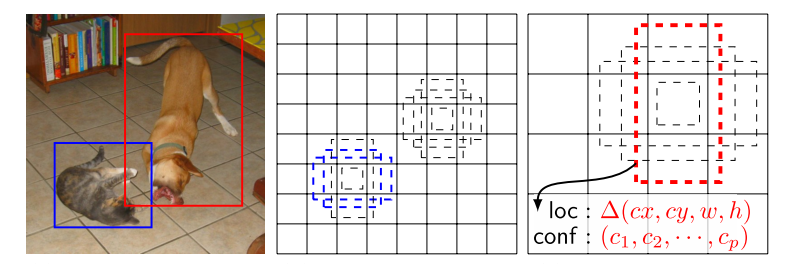
\includegraphics[width=0.9\textwidth]{fig/anchors}
	\caption{Illustration for anchor box concept \cite{ssd}}
	\label{fig:anchors}
\end{figure}
%----------------------------------------------------------------------------------------
\section{Architecture}

Usually a classification network like VGG-16 is used as \textit{base network}. On the final feature map additional convolutional layers are set, that predict class confidences and box coordinates. As for each anchor box a separate output is predicted, each predictor can "specialize" on objects that mostly fall in its aspect ratio/scale/ location (?). The networks implement the final predictions as 1x1 convolutions, thus realizing a fully connected layer more efficiently(?) and allowing various image sizes.

SSD adds several convolutional predictor layers that predict bounding boxes for various scales. They also use one lower layer of the base network for prediction as they assume it preserves more fine grained features.

The first Yolo version as displayed in \autoref{fig:architecture} used a fully connected layer as regression head. However, in the new version they also switched to one convolutional layer.

%----------------------------------------------------------------------------------------
\section{Training Goal}
SSDs treat object detection as a regression problem. The loss function usually incorporates the aforementioned bounding box coordinates and class scores. During training only one anchor box should be "responsible" for predicting that true box. This responsibility is determined by the location/size of the true box. The SSD paper refers to this as the \textit{matching strategy}.

Yolo matches those boxes to the ones that have their center at a certain grid cell. Among the remaining boxes the one with the highest intersection-over-union (IoU) is chosen. SSD matches anchor and true boxes only based on the IoU.

Yolo Prediction:
$$t_x,t_y,t_w,t_h,t_o \quad \text{from cell:} c_x, c_y$$

$$x = \sigma(t_x) + c_x \quad y = \sigma(t_y) + c_y \quad w = p_w e^{t_w} \quad h = p_he^{t_h \quad conf = \sigma(t_o)}$$
where $\sigma(x)$ is softmax function.
Yolo Loss:\\
$$ L = \lambda_{coord} \sum_{i=0}^{S^2}\sum_{j=0}^{B} 1^{obj}_{ij}(x_i - \hat{x}_i)^2 + (y_i - \hat{y_i})+$$
$$
\lambda_{coord} \sum_{i=0}^{S^2}\sum_{j=0}^{B} 1^{obj}_{ij}(\sqrt{w_i} - \sqrt{\hat{w}_i})^2 + (\sqrt{h_i} - \sqrt{\hat{h}_i})^2 +$$ 
$$\sum_{i=0}^{S^2}\sum_{j=0}^{B} 1^{obj}_{ij} (C_i - \hat{C_i})^2
+ 
\lambda_{noobj} \sum_{i=0}^{S^2}\sum_{j=0}^{B} 1^{noobj}_{ij} (C_i - \hat{C_i})^2
+ $$$$
\sum_{i=0}^{S^2}i_i^{obj} \sum_{c \in classes}(p_i(c) - \hat{p_i}(c))^2$$

SSD Loss:\\
$$L(x,c,l,g) = \frac{1}{N} (L_{conf}(x,c) +\alpha L_{loc}(x,l,g)$$\\
$$L_{loc}(x,l,g) = \sum_{i \in Pos}\sum_{m \in {cx,cy,w,h}} x_{ij}^k smooth_{L1} (l_i^m - \hat{g}^m_j)$$\\
$$\hat{g_j}^{cx} = (g_j^{cx} - d_i^{cx})/d_i^{w} \quad \hat{g_j}^{cy} = (g_j^{cy} - d_i^{cy})/d_i^{h}$$\\
$$\hat{g}_j^w = log(\frac{g_j^w}{d_i^w}) \quad \hat{g}_j^h = log(\frac{g_j^h}{d_i^h})$$

$$L_{conf}(x,c) = - \sum_{i \in Pos}^{N} x_{ij}^p log(\hat{c}_i^p) - \sum_{i \in Neg} log(\hat{c_i}^0) \quad \hat{c_i}^p = \frac{exp(c_i^p)}{\sum_{p} exp(c_i^p)}$$
\subsection{Negatives}

%----------------------------------------------------------------------------------------
\section{Data Augmentation}

\section{Comparison}
\subsection{Yolo}
\begin{enumerate}
	\item Only one convolutional layer for prediction
	\item Anchor boxes determined in pre-clustering step
\end{enumerate}
\subsection{SSD}
\begin{enumerate}
	\item 6 Convolutional layers
\end{enumerate}
%	BIBLIOGRAPHY
%----------------------------------------------------------------------------------------

\bibliographystyle{abbrv}

\bibliography{bib}

%----------------------------------------------------------------------------------------


\end{document}